\documentclass[DIV=16,parskip]{scrartcl} % siehe <http://www.komascript.de>
\usepackage{selinput} % Eingabecodierung automatisch ermitteln
\SelectInputMappings{ % siehe <http://ctan.org/pkg/selinput>
  adieresis={ä},
  germandbls={ß}
}
\setcounter{secnumdepth}{0}
\usepackage[ngerman]{babel}% Das Beispieldokument ist in Deutsch,
                % daher wird mit Hilfe des babel-Pakets
                % über Option ngerman auf deutsche Begriffe
                % und gleichzeitig Trennmuster nach den
                % aktuellen Rechtschreiberegeln umgeschaltet.
                % Alternativen und weitere Sprachen sind
                % verfügbar (siehe <http://ctan.org/pkg/babel>).
								
% Zeichensatz Latin Modern
\usepackage{lmodern}
\renewcommand*\familydefault{\sfdefault} %% Only if the base font of the document is to be sans serif
\usepackage[T1]{fontenc}

% Für Grafiken
\usepackage{graphicx}
\usepackage[absolute]{textpos}

% Für Formatierung von Tabellen
\usepackage{tabu}

% Für Mathematik
\usepackage{amsmath}

% Für mehr Flexibilität bei Aufzählungen
\usepackage{enumerate}
\usepackage{enumitem}

\usepackage{minted}

\usepackage{tikz}
\usetikzlibrary{arrows,automata}

\begin{document}

% FH Aachen Logo nach rechts oben in die Ecke der ersten Seite
%\begin{textblock*}{15mm}[1,0](210mm,10mm)
%	
\includegraphics[width=15mm]{img/logo.png}
%\end{textblock*}

\begin{flushleft}
{\footnotesize{Prof.\,Dr.\,A.\,Hannig \textbar{ }FH Aachen}} \\

\vspace{24pt}
\parindent=-0.5pt
\begin{tabu} {@{}X[l]X[c]X[r]@{}}
{\LARGE{\textbf{Datenbanken und Webtechnologien}}} & {\Large{WS1920}} & {\textnormal{Klausur 09.07.2020}} \\
\end{tabu}
\end{flushleft}

\vspace{24pt}

\newcommand{\udensdash}[1]{%
    \tikz[baseline=(todotted.base)]{
        \node[inner sep=1pt,outer sep=0pt] (todotted) {#1};
        \draw[densely dashed] (todotted.south west) -- (todotted.south east);
    }%
}%

\subsection{Aufgabe 1: HTML}
\label{sec:Aufgabe1}
\begin{enumerate}[label=\alph*)]
    \item Was ist ein Pseudoelement? (\textbf{multiple chioce})
    \item Wie sehen Kommentare in HTML? (\textbf{multiple chioce})
    \item ??? (\textbf{multiple chioce})
    \item Wie sieht der zugehörige HTML-Code aus? \\
        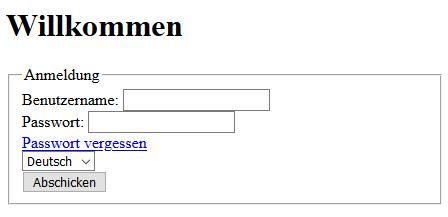
\includegraphics[width=15cm]{img/klausur.JPG}
        \begin{enumerate}[label=\arabic*.]
            \item Die Parameter sollen als "benutzername", "passwort" und "sprache"
                beim Server abfragbar sein.
            \item Benutzername ist max. 80 Zeichen lang und muss immer angegeben werden.
            \item Passwort soll nicht lesbar sein.
            \item Passwort vergessen leitet nach "/passwortzuruecksetzen" weiter.
            \item Sprache Deutsch soll standardmäßig aktiv sein. Die andere Option
                ist Englisch.
            \item Das Formular soll an /auswertung.php geschickt werden und mit
                \$\_POST ausgelesen werden können.
         \end{enumerate}
    \item Nennen Sie 4 Statuscodes samt Bedeutung.
    \item Nennen Sie 4 HTTP Methoden samt Bedeutung.
\end{enumerate}

\newpage
\subsection{Aufgabe 2: PHP}
\label{sec:Aufgabe2}
\begin{enumerate}[label=\alph*)]
    \item Gegeben ist folgendes Array in PHP. Schreiben Sie eine Funktion, so dass der angegebene HTML-Code dabei heraus kommt.
        \begin{minted}{php}
            array = [
                1 => 'a',
                2 => ['b', 'c'],
                3 => [4, 5, 6]
            ];
        \end{minted}
    
        \begin{minted}{html}
            <ol>
                <li> 1: a </li>
                <li> 2:
                    <ul>
                        <li> b </li>
                        <li> c </li>
                    </ul>
                </li>
                <li> 3:
                    <ul>
                        <li> 4 </li>
                        <li> 5 </li>
                        <li> 6 </li>
                    </ul>
                </li>
            </ol>
        \end{minted}
    \item Mit welchen Tag beginnt ein PHP-Script? (\textbf{multiple chioce})
    \item Wie inkludiere ich in PHP ein File? (\textbf{multiple chioce})
    \item Wie erhalte ich den HTTP-Header??? (\textbf{multiple chioce})
        \begin{enumerate}[label=\arabic*.]
            \item GET
            \item REQUEST
            \item POST
        \end{enumerate}
    \item Welche Aussagen sind in PHP true? (\textbf{multiple chioce})
        \begin{enumerate}[label=\arabic*.]
            \item \grqq 5.1\grqq == 5 
            \item 5 == \grqq 5.1\grqq
            \item \grqq true\grqq == \grqq true\grqq
            \item TRUE = 3
        \end{enumerate}
\end{enumerate}

\newpage
\subsection{Aufgabe 3: Normalisierung}
\label{sec:ex3}
\begin{enumerate}[label=\alph*)]
        % give item a label to point to it in the caption
    \item  Überführen Sie die folgende Tabelle in die 1NF.\label{itm:a3-first}\\
        %\\[2ex]  skips two lines
        \begin{table}[h!]
            \centering
            \begin{adjustbox}{max width=\textwidth}
                \begin{tabular}{*{4}{|c}|} % creates table with 4 columns
                    \hline % draws a horizontal line
                    \textbf{Artikel} & \textbf{Anschrift} & 
                    \textbf{Organisationsname} & \textbf{Lieferzeitpunkt}\\
                    \hline
                    502 Computer & 52070; Eupener Straße; 70 & Fh-Aachen & Vormittags; 
                    Nachmittags\\
                    \hline
                \end{tabular}
            \end{adjustbox}
            \caption{Ausgangstabelle für \ref{itm:a3-first}}
            \label{tab:transfrom_to_1nf}
        \end{table}
    \item Überführen Sie folgende Tabelle direkt in die 3NF. Unterstreichen Sie
        jeweils den \underline{Primärschlüssel} und den \dashuline{Fremdschlüssel}
        .\label{itm:a3-second}\\
        \begin{table}[h!]
            \centering
            \begin{adjustbox}{max width=\textwidth}
                \begin{tabular}{*{8}{|c}|} % draws seven columns
                    \hline
                    \textbf{Hersteller} & \textbf{Farbe} & \textbf{Knz} & \textbf{Farbcode}
                    & \textbf{Herstellersitz} & \textbf{Fahr\_Nr} & \textbf{Fahr\_Vorname}
                    & \textbf{Fahr\_Nachname}\\
                    \hline
                    Opel & Silber & DB-WT-10 & 135 & Rüsselsheim & 13337 & Ronnie & Nator\\
                    \hline
                    Opel & Blau & DB-WT-11 & 274 & Rüsselsheim & 13338 & Mike & Mann\\
                    \hline
                    VW & Beige & DB-WT-12 & 271 & Wolfsburg & 13339 & Frauke & Frau\\
                    \hline
                \end{tabular}
            \end{adjustbox}
            \caption{Ausgangstabelle für \ref{itm:a3-second}}
            \label{tab:transform_to_3nf}
        \end{table}
    \item Welche Bedingungen müssen gelten, damit eine Tabelle in der 2NF vorliegt?
    \item Erklären Sie den Begriff der funktionellen Abhängigkeit und erläutern
        Sie diesen an einem Beispiel.
\end{enumerate}

\subsection{Aufgabe 4: (SQL)}
\label{sec:Aufgabe4}
\begin{tabular}{c|c}
     \textbf{InterpretID} & \textbf{Interpret} \\
     \hline
     1 & Name1 \\
     2 & Name2 \\
     3 & Name3
\end{tabular}

\begin{tabular}{c|c|c}
     \underline{\textbf{AlbumID}} & \textbf{Name} & \udensdash{InterpretID} & Erscheinungsdatum\\
     \hline
     1 & Name1 & 1 \\
     2 & Name2 & 1\\
     3 & Name3 & 1
\end{tabular}

\begin{tabular}{c|c|c}
     \underline{\textbf{TrackID}} & \textbf{Trackname} & \udensdash{AlbumID} & Duration & InterpretID? \\
     \hline
     1 & Name1 & 1 \\
     2 & Name2 & 1\\
     3 & Name3 & 1
\end{tabular}
\begin{enumerate}[label=\alph*)]
    \item Geben Sie allte Tracks mit Duration > 200 aus.
    \item Geben Sie die Länge jedes Albums (Summe über alle Titel des Albums) aus.
    \item Geben Sie alle Interpreten und - sofern vorhanden - auch die zugehörigen Alben aus.
    \item Geben Sie alle Interpreten aus, zu denen es kein Album gibt.
    \item Geben Sie alle Tracks aus, deren Länge größer als der Durchschnitt ist.
    \item Erzeugen Sie eine View '5laengstetracks', welche die 5 längsten Tracks des Albums mit der ID 1 ausgibt.
    \item Löschen Sie die erzeuge View.
\end{enumerate}
\subsection{Aufgabe 5: (ER-Diagramm)}
\label{sec:Aufgabe5}
\begin{enumerate}[label=\alph*)]
    \item \textit{Hier kommt die Aufgabe}
\end{enumerate}
\newpage
\subsection{Aufgabe 6: XML}
\label{sec:Aufgabe6}
\begin{enumerate}[label=\alph*)]
    \item Gegeben ist folgendes XML. Wie sieht das zugehörige DTD aus? (Auch hier kommt es zu Abweichungen aus der Klausur)
    \begin{minted}{XML}
        <buch>
            <inhalt>
                <prolog iid='i1'>
                    Hier stand etwas...
                </prolog>
                <hauptteil iid='i2'>
                    Hier stand etwas...
                </hauptteil>
                <schluss iid='i3'>
                    Hier stand etwas...
                </schluss>
            </inhalt>
            <kapitel kid='k1' iid='i1'>
                <einleitung seitenanzahl=5>
                    Hier stand etwas...
                </einleitung>
                <abschnitt seitenanzahl=12>
                    Hier stand etwas...
                </abschnitt>
                <abschnitt seitenanzahl=3>
                    Hier stand etwas...
                </abschnitt>
            </kapitel>
            <kapitel kid='k2'>
                <abschnitt seitenanzahl=2>
                    Hier stand etwas...
                </abschnitt>
                <abschnitt seitenanzahl=13>
                    Hier stand etwas...
                </abschnitt>
            </kapitel>
        </buch>
    \end{minted}
    
    \item Wann spricht man von wohlgeformten XML?
    \item Wie lauten die XPath Befehle für folgende Abfragen?
    \begin{enumerate}[label=\arabic*.]
        \item Geben Sie den Text aus der Einleitung des ersten Kapitels an.
        \item Aus wie vielen Seiten besteht das erste Kapitel?
        \item Geben Sie das letzte Kapitel aus.
    \end{enumerate}
\end{enumerate}

\subsection{Aufgabe 7: Serialisierbarkeit}
\label{sec:Aufgabe7}
\begin{enumerate}[label=\alph*)]
    \item Beschreiben Sie was man unter einem Deadlock versteht und wie es zu
        einem Deadlock kommen kann.
    \item Skizzieren Sie beispielhaft die Situation eines Deadlocks unter
        Verwendung von Transaktionen und Ressourcen.
    \item Nennen Sie die vier verschiedenen Isolationslevel. Man kann diese
        Einstellung in SQL anpassen. Nennen Sie den passenden Befehl.
    \item Skizzieren Sie die Dirty Read Problematik mit einfachen Transaktionen.
    \item Erstellen Sie zu folgendem Schedule den Konfliktgraph und die Konfliktmenge.\\
          Info: Hier war ein Schedule mit drei verschiedenen Variablen und vier
          verschiedenen Transaktionen gegeben. Er hat zu keinem Zykel geführt,
          hatte jedoch sehr viele Konflitke.
\end{enumerate}


\end{document}
